\documentclass[12pt, a4paper]{article}

% ── Shared preamble (src/lecturenotes.sty) ────────────────────────────────────
%   Packages, colors, boxes, \sol/\soleq and math macros all live in
%   src/*.sty. \input@path points LaTeX two folders up to find them.
\makeatletter
\def\input@path{{../../}}
\makeatother
\usepackage{lecturenotes}

% ── Local TikZ styles (match T03) ─────────────────────────────────────────────
\usetikzlibrary{decorations.pathreplacing}
\tikzset{
  neuron/.style={circle, draw=mainblue, fill=boxbg,
      minimum size=0.6cm, inner sep=0pt, thick, font=\scriptsize},
  input/.style={circle, draw=gray!60, fill=gray!15,
      minimum size=0.6cm, inner sep=0pt, thick, font=\scriptsize},
  hlnode/.style={fill=orange!30, draw=orange!80!black},
  wire/.style={gray!60, line width=0.5pt},
  hlwire/.style={mainblue, line width=1.3pt},
  layerlabel/.style={font=\small\itshape, gray},
  brace/.style={decorate, decoration={brace, amplitude=4pt}, thick, gray},
}

% ── Document ──────────────────────────────────────────────────────────────────
\begin{document}

\begin{center}
  {\LARGE \textbf{Section 4.1: Why Convolutional Networks?}} \\[0.3em]
  {\large\itshape The Limits of the MLP and Three Key Ideas} \\[0.5em]
  {\large AI-IM Class --- Lecture Notes}%
  \ifstudentmode
    \quad {\normalsize\color{gray}[Student Copy]}%
  \fi
\end{center}

\vspace{1em}
\hrule
\vspace{1.5em}

In Section 3.4 we built a complete classifier: a stack of fully connected
layers, a softmax output and the cross-entropy loss. Nothing in that recipe
says what the input features \emph{are}; an MLP accepts any vector $\bx$.
In this chapter the input is an \textbf{image}. We will see that an MLP
\emph{can} read an image, but that it does so in a very wasteful way, and
that three simple ideas fix the problem. Those three ideas define the
\textbf{convolutional neural network (CNN)}. In this section we
\begin{itemize}[nosep]
  \item describe how an image is stored as numbers,
  \item feed an image to an MLP and find three weaknesses,
  \item introduce the three ideas behind convolution: \emph{sparse
          interactions}, \emph{parameter sharing} and \emph{equivariance},
        and
  \item look briefly at where the idea came from.
\end{itemize}

% ══════════════════════════════════════════════════════════════════════════════
\section{Images as Data}

A \textbf{grayscale image} is a grid of numbers. Each number is a
\textbf{pixel} and gives the brightness at that location, usually an integer
from $0$ (black) to $255$ (white). Before training we normally rescale the
pixels to $[0, 1]$ by dividing by $255$.

\begin{figure}[H]
  \centering
  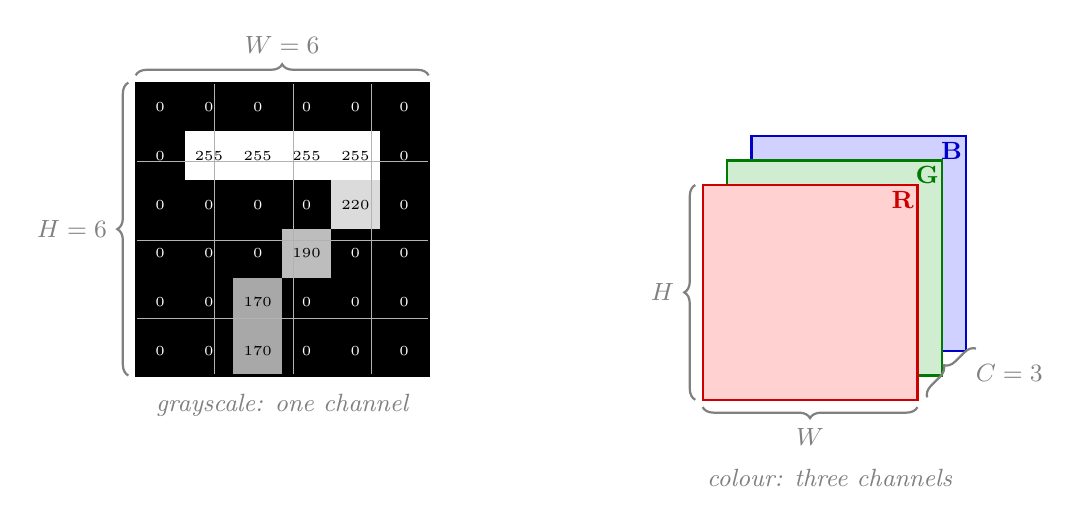
\begin{tikzpicture}[x=0.62cm, y=0.62cm]
    \foreach \row [count=\r] in {
        {0,0,0,0,0,0},
        {0,255,255,255,255,0},
        {0,0,0,0,220,0},
        {0,0,0,190,0,0},
        {0,0,170,0,0,0},
        {0,0,170,0,0,0}} {
        \foreach \v [count=\c] in \row {
            \pgfmathtruncatemacro{\p}{\v/255*100}
            \pgfmathtruncatemacro{\dark}{\v<128}
            \fill[white!\p!black] (\c-1, -\r+1) rectangle ++(1,-1);
            \ifnum\dark=1
              \node[font=\tiny, white] at (\c-0.5, -\r+0.5) {\v};
            \else
              \node[font=\tiny, black] at (\c-0.5, -\r+0.5) {\v};
            \fi
          }
      }
    \draw[gray!60] (0,0) grid (6,-6);
    \draw[thick] (0,0) rectangle (6,-6);
    \draw[brace] (0,0.15) -- node[above=4pt, font=\small] {$W = 6$} (6,0.15);
    \draw[brace] (-0.15,-6) -- node[left=4pt, font=\small] {$H = 6$} (-0.15,0);
    \node[layerlabel] at (3,-6.6) {grayscale: one channel};

    % ── colour image: three stacked channels ─────────────────────────────────
    \begin{scope}[xshift=7.2cm, yshift=-1.3cm]
      \foreach \col/\lbl/\s in {blue/B/2, green!60!black/G/1, red/R/0} {
          \filldraw[fill=\col!18, draw=\col!80!black, thick]
          (0.5*\s, 0.5*\s) rectangle ++(4.4, -4.4);
          \node[font=\small\bfseries, text=\col!80!black]
          at (0.5*\s+4.1, 0.5*\s-0.3) {\lbl};
        }
      \draw[brace] (4.4,-4.55) -- node[below=4pt, font=\small] {$W$} (0,-4.55);
      \draw[brace] (-0.15,-4.4) -- node[left=4pt, font=\small] {$H$} (-0.15,0);
      \draw[brace] (4.6,-4.35) -- node[right=5pt, font=\small] {$C = 3$}
      (5.6,-3.35);
      \node[layerlabel] at (2.6,-6.0) {colour: three channels};
    \end{scope}
  \end{tikzpicture}
  \caption{Left: a $6\times 6$ grayscale image of the digit ``7'' and its pixel
    values. Right: a colour image stores three such grids, one per
    \emph{channel} (red, green, blue).}
  \label{fig:image}
\end{figure}

A \textbf{colour image} stores three grids of the same size: one each for
the red, green and blue intensity. Each grid is a \textbf{channel}. So an
image is a three-dimensional array (a \emph{tensor}) with
\begin{itemize}[nosep]
  \item $C$ channels ($C = 1$ for grayscale, $C = 3$ for colour),
  \item height $H$ (number of rows), and
  \item width $W$ (number of columns).
\end{itemize}
We write the image as $\bX$ and its entries in lower case: $x_{i,j}$ is the
pixel in row $i$ and column $j$ (row $1$ is the top row).

\begin{notebox}
  \textbf{PyTorch convention.} PyTorch stores one image as a tensor of shape
  $(C, H, W)$, channels first. A mini-batch of $N$ images (Section 3.4) has
  shape $(N, C, H, W)$. A batch of 64 colour images of size
  $224 \times 224$ is therefore a tensor of shape $(64, 3, 224, 224)$.
  We use this order throughout the chapter.
\end{notebox}

\begin{stepbox}{Exercise 1 \quad How big is an image?}
  How many numbers are stored in each of the following?
  \begin{enumerate}[label=(\alph*), nosep]
    \item One MNIST digit, a grayscale image of $28 \times 28$ pixels:
          \quad $\sol[3cm]{28 \times 28 = 784}$
    \item One colour image of $224 \times 224$ pixels (a common input size
          for ImageNet models):
          \quad $\sol[5cm]{3 \times 224 \times 224 = 150\,528}$
    \item A batch of shape $(64, 3, 224, 224)$:
          \quad $\sol[5cm]{64 \times 150\,528 = 9\,633\,792}$
  \end{enumerate}
\end{stepbox}

% ══════════════════════════════════════════════════════════════════════════════
\section{Feeding an Image to an MLP}

An MLP expects a vector, so the obvious approach is to \textbf{flatten} the
image: read the pixels row by row and put them in one long column.
A $28 \times 28$ digit becomes a vector $\bx$ with $784$ entries, and the
MLP from Section 3.4 can classify it with $10$ softmax outputs.
This works reasonably well on MNIST (about 98\% test accuracy). It has three
weaknesses, and all three get worse as images become larger and more varied.

% ──────────────────────────────────────────────────────────────────────────────
\subsection{Weakness 1: Too Many Parameters}

Recall from Section 3.4 that a fully connected layer with $n_{\ell-1}$
inputs and $n_\ell$ nodes has $(n_{\ell-1} + 1)\,n_\ell$ parameters. With an
image as input, $n_0$ is the number of pixel values, which is large.

\begin{stepbox}{Exercise 2 \quad Parameters of the first layer}
  Count the parameters of the \emph{first} hidden layer only.
  \begin{center}
    \renewcommand{\arraystretch}{1.4}
    \begin{tabular}{lccc}
      \toprule
      Input                      & Inputs $n_0$          & Hidden nodes $n_1$ & Parameters                        \\
      \midrule
      MNIST, $1\times28\times28$ & $\sol[1.6cm]{784}$    & 128                & $\sol[3.2cm]{100\,480}$           \\
      Colour, $3\times224\times224$
                                 & $\sol[1.6cm]{150\,528}$
                                 & 1\,000             & $\sol[3.2cm]{150\,529\,000}$                            \\
      \bottomrule
    \end{tabular}
  \end{center}
\end{stepbox}

The second row has about \textbf{150 million} parameters in one layer. For
comparison, ResNet-50, a famous CNN that we meet in Section 4.4, has about
25 million parameters in its \emph{entire} network. Every parameter costs
memory and computation, and, more importantly, must be learned from data.
More parameters means more training images are needed before the model
stops fitting noise.

% ──────────────────────────────────────────────────────────────────────────────
\subsection{Weakness 2: Flattening Ignores Which Pixels Are Neighbours}

In an image, the pixels next to each other (left, right, above, below)
usually belong to the same object: an edge, a stroke, a corner. Flattening
destroys this layout. Two pixels that are vertically adjacent end up far
apart in the vector.

\begin{figure}[H]
  \centering
  \begin{tikzpicture}[x=0.6cm, y=0.6cm, >=Stealth]
    \foreach \r in {1,...,4} \foreach \c in {1,...,4} {
          \pgfmathtruncatemacro{\n}{(\r-1)*4+\c}
          \pgfmathtruncatemacro{\nb}{(\n==2)||(\n==5)||(\n==7)||(\n==10)}
          \ifnum\n=6
            \filldraw[fill=orange!70, draw=gray] (\c-1,-\r+1) rectangle ++(1,-1);
          \else\ifnum\nb=1
              \filldraw[fill=orange!20, draw=gray] (\c-1,-\r+1) rectangle ++(1,-1);
            \else
              \draw[gray] (\c-1,-\r+1) rectangle ++(1,-1);
            \fi\fi
          \node[font=\scriptsize] at (\c-0.5,-\r+0.5) {\n};
        }
    \node[layerlabel] at (2,-4.7) {$4\times4$ image};

    \draw[->, thick] (4.6,-2) -- node[above, font=\small] {flatten} (6.6,-2);

    \begin{scope}[xshift=4.4cm, yshift=-0.6cm]
      \foreach \n in {1,...,16} {
          \pgfmathtruncatemacro{\nb}{(\n==2)||(\n==5)||(\n==7)||(\n==10)}
          \ifnum\n=6
            \filldraw[fill=orange!70, draw=gray] (\n-1,0) rectangle ++(1,-1);
          \else\ifnum\nb=1
              \filldraw[fill=orange!20, draw=gray] (\n-1,0) rectangle ++(1,-1);
            \else
              \draw[gray] (\n-1,0) rectangle ++(1,-1);
            \fi\fi
          \node[font=\scriptsize] at (\n-0.5,-0.5) {\n};
        }
      \draw[<->, red!70!black, thick] (1.5,-1.2) to[bend right=25]
      node[below, font=\scriptsize] {4 apart} (5.5,-1.2);
      \draw[<->, red!70!black, thick] (5.5,-1.2) to[bend right=25]
      node[below, font=\scriptsize] {4 apart} (9.5,-1.2);
      \node[layerlabel] at (8,-3.1) {vector $\bx$ with 16 entries};
    \end{scope}
  \end{tikzpicture}
  \caption{Pixel 6 (dark) and its four neighbours (light). After flattening,
    only the left and right neighbours stay next to it. The neighbours above
    and below are a whole row ($W$ entries) away.}
  \label{fig:flatten}
\end{figure}

\begin{stepbox}{Exercise 3 \quad Where does a pixel go?}
  A $28 \times 28$ image is flattened row by row (this is what
  \texttt{torch.flatten} does). Number the entries of $\bx$ from $1$.
  \begin{enumerate}[label=(\alph*), nosep]
    \item The pixel in row $i$, column $j$ goes to position
          $\sol[3.5cm]{(i-1)\cdot 28 + j}$.
    \item Pixel $(3, 5)$ goes to position $\sol[1.5cm]{61}$. Its right
          neighbour $(3, 6)$ goes to $\sol[1.5cm]{62}$, and the pixel below it,
          $(4, 5)$, goes to $\sol[1.5cm]{89}$.
  \end{enumerate}
\end{stepbox}

The MLP does not use the layout at all. A thought experiment makes this
clear: pick one fixed random reordering of the 784 pixels and apply it to
every training and test image. To a human the images now look like noise.
The MLP, however, trains to \emph{exactly} the same accuracy, because a
fully connected layer treats its inputs as an unordered list. Reordering the
inputs only reorders the columns of $\bW^{(1)}$. Everything we know about
images (that nearby pixels go together) is thrown away and must be learned
again from data.

% ──────────────────────────────────────────────────────────────────────────────
\subsection{Weakness 3: A Pattern Learned in One Place Is Unknown Elsewhere}
\label{sec:bump}

A cat is a cat whether it sits on the left or the right of the photo.
For an MLP, the two cases are unrelated. We show this with the smallest
possible example: a one-dimensional ``image'' with seven pixels, containing
one bright pixel (a ``bump'').
\[
  \bx_A = (0,\, 0,\, 1,\, 0,\, 0,\, 0,\, 0),
  \qquad
  \bx_B = (0,\, 0,\, 0,\, 0,\, 1,\, 0,\, 0).
\]
Image $B$ is image $A$ shifted two pixels to the right. Suppose a hidden node
has learned to detect the bump in image $A$, with weights
\[
  \bw = (0,\, -1,\, 2,\, -1,\, 0,\, 0,\, 0), \qquad b = 0.
\]
The weight $+2$ rewards a bright centre pixel; the two $-1$ weights penalise
bright neighbours, so the node responds to an isolated bright point.

\begin{stepbox}{Exercise 4 \quad One node, two positions}
  Compute the pre-activation $z = \bw^\top \bx + b$ for both images.
  \[
    z_A = \sol[6cm]{(-1)(0) + (2)(1) + (-1)(0) = 2},
    \qquad
    z_B = \sol[3cm]{0}
  \]
\end{stepbox}

The node fires for image $A$ and is silent for image $B$, although both
contain the same bump. To detect the bump at every position, the MLP needs a
separate node for each position, each learning the \emph{same} pattern
$(-1, 2, -1)$ from its own examples. A CNN instead learns the pattern
once and reuses it everywhere.

% ══════════════════════════════════════════════════════════════════════════════
\section{Three Key Ideas}

The fix for the bump problem is to take the small pattern
$\bw = (w_1, w_2, w_3) = (-1, 2, -1)$, called a \textbf{kernel} (or
\textbf{filter}), and slide it along the input. At each position we compute
one weighted sum:
\begin{resultbox}
  \[
    z_i = w_1 x_i + w_2 x_{i+1} + w_3 x_{i+2},
    \qquad i = 1, 2, \dots
  \]
\end{resultbox}
This sliding weighted sum is the \textbf{convolution} that gives CNNs their
name. Section 4.2 defines it formally, including what happens at the borders.
For now we only need the formula above. With $7$ inputs and a kernel of width
$3$ there are $7 - 3 + 1 = 5$ positions, so we get $5$ outputs
$z_1, \dots, z_5$.

Compared with a fully connected layer, this layer has three properties that
make it a good fit for images (Goodfellow et al., \emph{Deep Learning},
Section 9.2).

% ──────────────────────────────────────────────────────────────────────────────
\subsection{Idea 1: Sparse Interactions}

In a fully connected layer, every output is connected to every input. In a
convolution, output $z_i$ is connected to only $k$ inputs, where $k$ is the
width of the kernel. The inputs that affect an output form its
\textbf{receptive field}. In Figure~\ref{fig:connectivity} the receptive field
of $z_2$ is $\{x_2, x_3, x_4\}$.

This matches what we know about images: small, useful features such as edges
and corners involve only a few neighbouring pixels, not the whole image.

% ──────────────────────────────────────────────────────────────────────────────
\subsection{Idea 2: Parameter Sharing}

In a fully connected layer every weight is used exactly once: it multiplies one
input to produce one output. In a convolution the \emph{same} $k$ weights are
used at every position. This is \textbf{parameter sharing} (also called
\emph{tied weights}). The layer learns one kernel instead of one set of
weights per location.

\begin{figure}[H]
  \centering
  \begin{tikzpicture}[x=0.68cm, y=1cm]
    % ── (a) dense ──────────────────────────────────────────────────────────────
    \foreach \i in {1,...,6} \node[input] (a\i) at (\i, 0) {$x_{\i}$};
    \foreach \j in {1,...,4} \node[neuron] (A\j) at (\j+1, 1.9) {$z_{\j}$};
    \foreach \j in {1,...,4} \foreach \i in {1,...,6} \draw[wire] (A\j) -- (a\i);
    \foreach \i in {1,...,6} \draw[hlwire] (A2) -- (a\i);
    \node[font=\small] at (3.5, -0.8) {(a) dense};

    % ── (b) local, not shared ─────────────────────────────────────────────────
    \begin{scope}[xshift=5.3cm]
      \foreach \i in {1,...,6} \node[input] (b\i) at (\i, 0) {$x_{\i}$};
      \foreach \j in {1,...,4} \node[neuron] (B\j) at (\j+1, 1.9) {$z_{\j}$};
      \foreach \j in {1,...,4} {
          \pgfmathtruncatemacro{\ja}{\j+1}
          \pgfmathtruncatemacro{\jb}{\j+2}
          \draw[wire] (B\j) -- (b\j);
          \draw[wire] (B\j) -- (b\ja);
          \draw[wire] (B\j) -- (b\jb);
        }
      \foreach \i in {2,3,4} {
          \node[input, hlnode] at (b\i) {$x_{\i}$};
          \draw[hlwire] (B2) -- (b\i);
        }
      \node[font=\small] at (3.5, -0.8) {(b) local};
    \end{scope}

    % ── (c) local and shared ──────────────────────────────────────────────────
    \begin{scope}[xshift=10.6cm]
      \foreach \i in {1,...,6} \node[input] (c\i) at (\i, 0) {$x_{\i}$};
      \foreach \j in {1,...,4} \node[neuron] (C\j) at (\j+1, 1.9) {$z_{\j}$};
      \foreach \j in {1,...,4} {
          \pgfmathtruncatemacro{\ja}{\j+1}
          \pgfmathtruncatemacro{\jb}{\j+2}
          \draw[red!70!black, line width=0.9pt] (C\j) -- (c\j);
          \draw[mainblue, line width=0.9pt] (C\j) -- (c\ja);
          \draw[green!50!black, line width=0.9pt] (C\j) -- (c\jb);
        }
      \node[font=\small] at (3.5, -0.8) {(c) local + shared};
      \node[font=\scriptsize, align=left, anchor=west] at (6.6, 1.0)
      {\textcolor{red!70!black}{$w_1$}\\
        \textcolor{mainblue}{$w_2$}\\
        \textcolor{green!50!black}{$w_3$}};
    \end{scope}
  \end{tikzpicture}
  \caption{Six inputs, four outputs. (a) A dense layer connects every output
    to every input. (b) Local connections: $z_2$ sees only its receptive field
    $x_2, x_3, x_4$. (c) Convolution: local connections that reuse the same
    three weights at every position (same colour = same weight).}
  \label{fig:connectivity}
\end{figure}

\begin{stepbox}{Exercise 5 \quad Counting weights}
  Count the weights (ignore biases) for the three layers in
  Figure~\ref{fig:connectivity}, then for general sizes: $m$ inputs, $n$
  outputs and kernel width $k$.
  \begin{center}
    \renewcommand{\arraystretch}{1.4}
    \begin{tabular}{lcc}
      \toprule
      Layer                  & $m = 6,\ n = 4,\ k = 3$ & General             \\
      \midrule
      (a) Dense              & $\sol[1.5cm]{24}$       & $\sol[2cm]{m n}$    \\
      (b) Local              & $\sol[1.5cm]{12}$       & $\sol[2cm]{k n}$    \\
      (c) Local + shared     & $\sol[1.5cm]{3}$        & $\sol[2cm]{k}$      \\
      \bottomrule
    \end{tabular}
  \end{center}
\end{stepbox}

Sparse interactions reduce the weights from $mn$ to $kn$; sharing reduces them
further to $k$, which no longer depends on the size of the image. The
following example from Goodfellow et al.\ shows how large the difference is
for a real photo.

\begin{stepbox}{Exercise 6 \quad Edge detection}
  The kernel $\bw = (-1, 1)$ computes $z_i = x_{i+1} - x_i$: each pixel minus
  its left neighbour.
  \begin{enumerate}[label=(\alph*)]
    \item Apply it to one row of an image,
          $\bx = (10, 10, 10, 80, 80, 80)$:
          \[
            \bz = \bigl(\,\sol[1cm]{0},\ \sol[1cm]{0},\ \sol[1cm]{70},\
            \sol[1cm]{0},\ \sol[1cm]{0}\,\bigr)
          \]
          The output is non-zero only at the jump from dark to bright: the
          kernel is a \textbf{vertical edge detector}.
    \item Now apply it to every row of a photo that is $280$ pixels tall
          and $320$ pixels wide. Each row gives $319$ outputs, so the output
          image has $280 \times 319 = \sol[2.2cm]{89\,320}$ pixels.
    \item Each output costs two multiplications and one addition. The whole
          convolution costs $\sol[2.2cm]{267\,960}$ operations and has only
          $\sol[1cm]{2}$ parameters.
    \item A dense layer that computes the same output needs one weight per
          (input, output) pair:
          \[
            (280 \times 320) \times (280 \times 319)
            = \sol[7cm]{89\,600 \times 89\,320 \approx 8.0 \times 10^{9}}
            \ \text{weights.}
          \]
  \end{enumerate}
\end{stepbox}

Over eight billion weights, almost all of them zero, to describe what two
numbers describe. Convolution is an extremely compact way to apply
\emph{the same small, local operation everywhere} in an image.

% ──────────────────────────────────────────────────────────────────────────────
\subsection{Idea 3: Equivariance to Translation}

Return to the bump images $\bx_A$ and $\bx_B$ of
Section~\ref{sec:bump}. Instead of one dense node, use the sliding kernel
$\bw = (-1, 2, -1)$.

\begin{stepbox}{Exercise 7 \quad Slide the kernel}
  Compute $z_i = -x_i + 2x_{i+1} - x_{i+2}$ for $i = 1, \dots, 5$.
  \begin{center}
    \renewcommand{\arraystretch}{1.4}
    \begin{tabular}{l*{7}{c}}
      \toprule
      $i$             & 1  & 2  & 3  & 4  & 5  & 6  & 7  \\
      \midrule
      $x_{A,i}$       & 0  & 0  & 1  & 0  & 0  & 0  & 0  \\
      $z_{A,i}$       & $\sol[0.8cm]{-1}$ & $\sol[0.8cm]{2}$ & $\sol[0.8cm]{-1}$
                      & $\sol[0.8cm]{0}$  & $\sol[0.8cm]{0}$ & --- & ---       \\
      \midrule
      $x_{B,i}$       & 0  & 0  & 0  & 0  & 1  & 0  & 0  \\
      $z_{B,i}$       & $\sol[0.8cm]{0}$  & $\sol[0.8cm]{0}$ & $\sol[0.8cm]{-1}$
                      & $\sol[0.8cm]{2}$  & $\sol[0.8cm]{-1}$ & --- & ---      \\
      \bottomrule
    \end{tabular}
  \end{center}
  The bump in $B$ is two pixels to the right of the bump in $A$. The output
  $\bz_B$ is $\bz_A$ shifted $\sol[2.5cm]{\text{two pixels to the right}}$.
\end{stepbox}

The same kernel finds the bump at both positions, and the output tells us
\emph{where} it is. This property has a name.

\begin{resultbox}
  A function $f$ is \textbf{equivariant} to a transformation $g$ if
  applying $g$ before or after $f$ gives the same result:
  \[
    f\bigl(g(\bx)\bigr) = g\bigl(f(\bx)\bigr).
  \]
  Convolution is equivariant to \textbf{translation} (shifting): shift the
  input, and the output shifts by the same amount.
\end{resultbox}

In two dimensions, the output of a convolution is a \textbf{feature map}: a
2-D map showing where a feature (such as a vertical edge) appears in the image.
If the object moves, its features move by the same amount in the map.

\paragraph{Equivariance vs.\ invariance.}
For classification we eventually want a stronger property. The answer
``cat'' should not change at all when the cat moves. A function is
\textbf{invariant} to $g$ if $f(g(\bx)) = f(\bx)$. Convolution alone is
equivariant, not invariant, but one extra step makes it invariant.

\begin{stepbox}{Exercise 8 \quad From equivariant to invariant}
  Summarise each feature map from Exercise 7 by its largest value:
  \[
    \max_i z_{A,i} = \sol[1cm]{2},
    \qquad
    \max_i z_{B,i} = \sol[1cm]{2}.
  \]
  The summary answers ``is there a bump?'' and gives the same answer for both
  positions.
\end{stepbox}

Taking a maximum over a region is called \textbf{pooling}, and it is the
topic of Section 4.3. The two steps divide the work: convolution detects
features wherever they are, and pooling discards their exact position.

\begin{notebox}
  \textbf{What convolution does \emph{not} give.}
  Convolution is equivariant to shifts only. It is not naturally equivariant
  to rotation or to a change of scale: a kernel that detects vertical edges
  does not detect horizontal ones. CNNs handle these variations by learning
  many kernels (Section 4.2) and by training on rotated and rescaled
  copies of the images.
\end{notebox}

% ──────────────────────────────────────────────────────────────────────────────
\subsection{Deeper Layers See More}

Sparse interactions do not mean that the network only ever looks at small
regions. If we stack convolutional layers, each output of the second layer
depends on several outputs of the first, which together cover a wider part of
the input.

\begin{figure}[H]
  \centering
  \begin{tikzpicture}[x=1.05cm, y=1.25cm]
    \foreach \i in {1,...,7} \node[input] (x\i) at (\i, 0) {$x_{\i}$};
    \foreach \j in {1,...,5} \node[neuron] (h\j) at (\j+1, 1) {$h_{\j}$};
    \foreach \k in {1,...,3} \node[neuron] (g\k) at (\k+2, 2) {$g_{\k}$};
    \foreach \j in {1,...,5} {
        \pgfmathtruncatemacro{\ja}{\j+1}
        \pgfmathtruncatemacro{\jb}{\j+2}
        \draw[wire] (h\j) -- (x\j); \draw[wire] (h\j) -- (x\ja);
        \draw[wire] (h\j) -- (x\jb);
      }
    \foreach \k in {1,...,3} {
        \pgfmathtruncatemacro{\ka}{\k+1}
        \pgfmathtruncatemacro{\kb}{\k+2}
        \draw[wire] (g\k) -- (h\k); \draw[wire] (g\k) -- (h\ka);
        \draw[wire] (g\k) -- (h\kb);
      }
    % highlight the receptive field of g2
    \foreach \j in {2,3,4} {
        \node[neuron, hlnode] at (h\j) {$h_{\j}$};
        \draw[hlwire] (g2) -- (h\j);
        \pgfmathtruncatemacro{\ja}{\j+1}
        \pgfmathtruncatemacro{\jb}{\j+2}
        \draw[hlwire] (h\j) -- (x\j); \draw[hlwire] (h\j) -- (x\ja);
        \draw[hlwire] (h\j) -- (x\jb);
      }
    \foreach \i in {2,...,6} \node[input, hlnode] at (x\i) {$x_{\i}$};
    \node[neuron, fill=mainblue!40] at (g2) {$g_2$};

    \node[layerlabel, anchor=west] at (8.0, 0) {input};
    \node[layerlabel, anchor=west] at (8.0, 1) {layer 1 (kernel 3)};
    \node[layerlabel, anchor=west] at (8.0, 2) {layer 2 (kernel 3)};
  \end{tikzpicture}
  \caption{Two stacked convolutions, each with kernel width $3$. Unit $g_2$
    is directly connected to only three units of layer 1, but indirectly
    depends on five inputs, $x_2, \dots, x_6$.}
  \label{fig:receptive}
\end{figure}

\begin{stepbox}{Exercise 9 \quad Growing receptive field}
  Each layer uses a kernel of width $3$. Fill in the width of the receptive
  field (measured on the input) of one unit in layer $L$.
  \begin{center}
    \renewcommand{\arraystretch}{1.4}
    \begin{tabular}{l*{5}{c}}
      \toprule
      Layer $L$        & 1 & 2 & 3                & 10                & $L$                 \\
      \midrule
      Receptive field  & 3 & 5 & $\sol[1cm]{7}$   & $\sol[1cm]{21}$   & $\sol[1.5cm]{2L+1}$ \\
      \bottomrule
    \end{tabular}
  \end{center}
  With kernels of width $k$, each layer adds $k-1$, so the receptive field is
  $\sol[2.5cm]{1 + L(k-1)}$.
  How many layers of width $3$ are needed before one unit sees a whole MNIST
  row of $28$ pixels? \quad $\sol[3cm]{2L+1 \ge 28 \Rightarrow L = 14}$
\end{stepbox}

Fourteen layers just to see one row is slow growth. Pooling and strides
(Sections 4.2 and 4.3) make the receptive field grow much faster. The
picture of a deep CNN that emerges is a hierarchy: early layers detect edges
in small patches, middle layers combine edges into textures and parts, and
late layers, which see most of the image, combine parts into objects.

% ══════════════════════════════════════════════════════════════════════════════
\section{Where the Idea Came From}

CNNs were inspired by the \textbf{visual cortex}, the part of the brain that
processes what the eyes see.
\begin{itemize}
  \item In the late 1950s and 1960s, David Hubel and Torsten Wiesel recorded
        single neurons in the visual cortex of cats. Each neuron responded
        only to stimuli in a small region of the visual field (a
        \emph{local receptive field}), and many responded only to edges of a
        particular orientation. \emph{Simple cells} reacted to an edge at an
        exact position; \emph{complex cells} reacted to the same edge
        anywhere in a small region. These correspond to convolution and
        pooling. The work earned the 1981 Nobel Prize in Medicine.
  \item In 1980 Kunihiko Fukushima built the \textbf{Neocognitron}, a network
        of alternating ``simple'' and ``complex'' layers, but without
        gradient-based training.
  \item In 1989 Yann LeCun and colleagues trained a convolutional network with
        backpropagation to read handwritten ZIP codes. This led to
        \textbf{LeNet-5} (1998), which read cheques in US banks.
  \item In 2012 \textbf{AlexNet} won the ImageNet challenge by a wide margin
        using GPUs, and CNNs became the standard approach to computer vision.
\end{itemize}

\begin{figure}[H]
  \centering
  \begin{tikzpicture}[x=0.25cm, >=Stealth]
    \draw[->, thick, gray] (0,0) -- (60,0);
    \foreach \yr/\lbl/\pos in {
        1959/{Hubel \& Wiesel}/above,
        1980/Neocognitron/below,
        1989/{LeCun: CNN +\\backprop}/above,
        1998/LeNet-5/below,
        2012/AlexNet/above} {
        \pgfmathsetmacro{\xx}{\yr-1955}
        \fill[mainblue] (\xx,0) circle (3pt);
        \node[\pos=3pt, font=\scriptsize, align=center] at (\xx,0)
        {\textbf{\yr}\\\lbl};
      }
  \end{tikzpicture}
  \caption{From neuroscience to deep learning.}
  \label{fig:timeline}
\end{figure}

\begin{notebox}
  \textbf{Inspiration, not imitation.} A CNN is not a model of the brain.
  The useful lesson from biology is the \emph{design}: local receptive fields,
  the same detector repeated across the visual field, and a hierarchy from
  simple to complex features. These are exactly Ideas 1--3.
\end{notebox}

% ══════════════════════════════════════════════════════════════════════════════
\section{Summary}

\begin{center}
  \renewcommand{\arraystretch}{1.35}
  \begin{tabular}{>{\raggedright\arraybackslash}p{5.2cm}
      >{\raggedright\arraybackslash}p{3.6cm}
      >{\raggedright\arraybackslash}p{5.6cm}}
    \toprule
    MLP weakness                                & Idea               & Effect                                              \\
    \midrule
    Every pixel connects to every node          & Sparse interactions & Each output sees a small receptive field            \\
    Separate weights for every position         & Parameter sharing   & One kernel of $k$ weights, independent of image size \\
    Pattern must be relearned at each position  & Equivariance        & Shift the input, the feature map shifts with it     \\
    \bottomrule
  \end{tabular}
\end{center}

\begin{itemize}
  \item An image is a tensor of shape $(C, H, W)$; a batch has shape
        $(N, C, H, W)$ in PyTorch.
  \item Flattening an image into an MLP creates a huge first layer, ignores
        which pixels are neighbours, and forces every pattern to be learned
        again at every position.
  \item A convolution slides one small kernel across the input:
        $z_i = w_1 x_i + w_2 x_{i+1} + \dots + w_k x_{i+k-1}$.
  \item Convolution is equivariant to translation; adding pooling makes the
        result (approximately) invariant.
  \item Stacking layers enlarges the receptive field, giving a hierarchy of
        edges $\to$ parts $\to$ objects.
\end{itemize}

\paragraph{Coming up.}
Section 4.2 defines convolution in 1-D and 2-D, with padding, stride and
multiple channels, and computes its gradient. Section 4.3 adds pooling and
assembles a complete CNN. Section 4.4 studies famous architectures from
LeNet-5 to ResNet, and Section 4.5 looks beyond classification at object
detection and OCR.

\end{document}
